\documentclass[a4paper, lualatex]{bxjsarticle}


%package
\usepackage{luatexja}
\usepackage{luatexja-fontspec}
\usepackage{unicode-math}
\usepackage{graphicx, xcolor, amsmath, cite, ascmac, amsfonts}


%other command
\makeatletter
\newcommand{\tref}[1]{Table.~\ref{#1}}
\newcommand{\eref}[1]{Eq.~(\ref{#1})}
\newcommand{\fref}[1]{Fig.~\ref{#1}}
\renewcommand{\theequation}{
  \thesection.\arabic{equation}}
\@addtoreset{equation}{chapter}
\def\cite#1{\textsubscript{#1}}
%\def\section{\newpage\@startsection {section}{2}{\z@}{3truemm}{3truemm}{\Large\bf}}
\makeatother
%\AtBeginSection[]{
%  \frame{\tableofcontents[currentsection, hideallsubsections]}
%}


\title{周期ポテンシャルに入射した波束の時間発展}
\author{前田大輝}
\begin{document}
\maketitle
\tableofcontents
\begin{section}{概要}
    \par Schrödinger方程式に従う量子波束について、Kronig-Penny型の副格子を持つステップ型ポテンシャルから作用を受けた場合の時間発展を数値計算によってシミュレートし多角的な解析を試みた。反射率と副格子の構造との関係について、壁が厚くなるごとに一定時間後の反射率が低下する場合が有ることをみいだした。また、確率分布の時空間的構造の解析から、非線形効果を取り入れていないにも関わらず、透過波束が二つ以上の波束に分裂する現象等をみいだした。
    \par また、多様なポテンシャルについて統一的に解析を行うため、汎用ポテンシャルに対する数値計算を行うフレームワークを作成した。このフレームワークは多様な物理的状況について手軽にシミュレーションを行うことが出来る。
\end{section}
\begin{section}{研究の背景と目的}
    \par 周期ポテンシャルは結晶中によく現れることから、物性物理学における重要な研究対象となっている。 歴史的にはBlochによって周期ポテンシャルが持つ並進対称性を利用した理論が作られ、結晶理論の基礎となっている。この理論の簡単で有効な実例としてKronig-Pennyモデルによるエネルギーバンド構造の説明が知られている。 また、準結晶のように並進対称性が部分的に破れている場合はAnderson局在を考慮に入れる理論がよく現実を説明できる近似として用いられている。 さらに、真空中から結晶中に入射する場合のように並進対称性が大きく破れている場合は転送行列を直接用いることで反射率や透過率を求められる場合がある。
    \par このように周期ポテンシャルにおける定常状態についてはかなり広い場合について理論的に基礎付けられている。非定常状態もこれらの定常状態を重ねあわせることで記述可能だが、波束のように局在化している場合は波動関数が周期性を持たない。よって、無限に長い波長を持つ固有状態にわたって積分する必要があり、解析的に解ける場合は限られている。
    \par しかしながら、近年では上記の理論に直接基礎付けられていない方法での解析技術も生まれている。
    \par 例えば、実験的方法が可能となっている。BECによる物質波波束を構成する方法が確立されている。また、レーザ技術の発展によって周期ポテンシャルを構成する技術も確立されている。
    \par ポテンシャル制御技術については、光格子時計のように高度に制御された場を作ることが可能になっている。これによって時間分解能の向上という時間発展の解析に必要な副次的技術も向上している。
    \par また、理論的な研究も行われている。周期結晶や準結晶中の波束について、Zhangによるモデル計算が行われ、波束の存在確率の分散が時間の3乗程度に比例して増大する場合が発見されている。
    \par 通常の真空中におけるGauss型波束は時間の2乗に比例して分散が増大するため、真空中よりも高次の拡散が起こっている。一般にブラウン運動よりも高次の拡散はHeyperdiffusionとして知られている。
    \par Zhangの研究の様に量子波束の時間発展では興味深い現象が起こり得るが、標準的なモデルがなく数値計算でSchrödinger方程式を直接解くという方法が取られている。
    \par 本研究では真空中からKronig-Penny型の周期ポテンシャル中に入射する粒子という並進対称性が大きく崩れた場合を扱う。
    \par このような場合にでも有効な数値計算法を確立すること、波束についての興味深い現象を発見することが本研究の目的となる。
\end{section}
\begin{section}{方法}
    \par 本研究では真空中からKronig-Penny型のポテンシャルに入射する波束の時間発展を数値計算によって解析した。数値計算には自作の数値計算フレームワークであるQuantumSketchBook(QSB)を作成し、使用した。本章では、使用したポテンシャルとパラメータの説明を行い、次に作成したフレームワークの説明と妥当性の検証を行う。
    \begin{subsection}{Kronig-Pennyモデルについて}
        \par 非相対論的な電子の確率振幅$\psi(x,t)$はSchrödinger方程式に従うことが知られている。
        \begin{align}
         i \frac{\partial}{\partial t}\psi(x, t) &= H \psi(x, t)\nonumber\\
             H &= -\frac{1}{2}\Delta + V(x)
        \end{align}
        \par ただし原子単位系を用いて、$\hbar=m=1$としている。Schrödinger方程式は波動方程式型の微分方程式であり、物理的状況に応じてポテンシャル$V(x)$と境界条件を与えることで解が決定する。
        \par 最も簡単なポテンシャルとしてステップ型、箱型、井戸型のポテンシャルが入門的な教科書によく取り入れられている。これらの単純なポテンシャルであっても、トンネル効果等の重要な現象を予言することが出来るため、モデルとしても一定の価値を持っている。
        \par 結晶を構成する原子が極めて周期的に並んでいるという事実を反映させたものとして周期ポテンシャルが使われる。周期$l$を持つポテンシャル$V_{periodic}$は以下の式に従う。
        \begin{align}
         V_{periodic}(x)=V_{periodic}(x-l)\nonumber\\
        \end{align}
        \par ポテンシャルが周期性を持つことから、系全体が並進対称性を持つことが言えるため、定常状態の確率振幅$\phi(x)$についてはBlochの定理が成立する。
            \begin{align}
             \phi(x)=u(x)\mathrm{e}^{-iKx}\nonumber\\
            \end{align}
        \end{subsection}
        \par $u(x)$はポテンシャルと同じ周期を持ち、系の構造に依存する関数でBloch関数と呼ばれる。$K$はポテンシャルの周期に依存する定数で逆格子定数と呼ばれる。逆格子定数はポテンシャルの周期の間に以下の関係が有る
        \begin{align}
         Kl&=2n\pi\nonumber\\
            n&\in \mathbb{N}
        \end{align}
        \par Blochの定理が成立する場合について最も早くから定常解が知られているものの一つとしてKronig-Pennyモデルがある。Kronig-Pennyモデルは箱型ポテンシャルが周期的に並んだモデルとして定義される。ポテンシャルが高い部分のことを壁(barrier)と呼び、ポテンシャルが低い部分のことを井戸(well)と呼ぶ。
        \begin{align}
         V_{kp}&=\begin{cases}V_0&(0\gt\ x\ \ge a)\\ 0&(a\gt\ x\ge\ l)\end{cases}\nonumber\\
            V_{KP}(x)&=V_{KP}(x-l)
        \end{align}
        \par ただし、壁の厚さを$a$周期を$l$と置いている。自動的に井戸の幅は$b=l-a$となる。Kronig-Pennyポテンシャルは$V_0$, $a$, $b$ の3つのパrメータによって特徴づけられる。
        \par 波動関数に$C^2$級の制限を加えるとKronig-Pennyモデルの定常解が得られる。定常解は禁止帯を持つことから、エネルギーバンド構造を表現することができている。
        \par 周期的に並べることが出来るものの中で最も簡単なポテンシャルである箱型ポテンシャルを周期的に並べただけという点がKronig-Pennyモデルの重要な特徴といえる。
        \par この単純さのお陰で、最も単純にエネルギーバンドを説明できるモデルの一つとしての教育的な価値が認められている。
        \par また、ポテンシャルが完全に局在化しているため、反射、透過の定義が有限の位置で可能であるという特質も持っている。
    \end{section}
    \begin{subsection}{QSBについて}
        \par QSBはSchrödinger方程式系の求解、可視化のためのフレームワークとして設計されている。使用の対象者として、数値計算に不慣れな物理学者を想定している。理解しやすくするために、データ構造に物理的な対応物を与えている点が特徴で、このような設計方法はオブジェクト指向(Object Oriented Programing:OOP)と呼ばれている。
        \par 本質的ではない環境構築等の手間を少なくするため、pythonでの実装を行っている。
        pythonには以下のような性質があり、今回のようなフレームワーク作成に適している。
        \begin{itemize}
            \item 環境整備が簡単で無償(mac等ではプリインストールされている)
            \item マルチパラダイム言語(手続き指向、オブジェクト指向、関数指向に対応している)
            \item 充実した科学計算系のライブラリ(numpy, scipy, matplotlib)
        \end{itemize}
        \par 特に科学計算系のライブラリとしてnumpyおよび、それを内包したscipyが線形代数、特殊関数、数値積分、微分、補間、並列計算等の計算を網羅的にサポートしている。
        \par pythonの処理系はc,Fortranに比べて一般に低速だが、scipyは実質的な計算処理を高度に最適化されたFortranサブモジュールのBLASS,LAPACK等に移譲することで高速な計算を可能としている。
        \par ただし、機能を最大限に利用するためにはpythonネイティブのループを用いない等の最適化が必要で、本質的ではないノウハウが必要となる。
        \par また、連続量の離散化など、定型的で退屈な処理はコードの可読性を悪化させる。
        \par そこで、ある程度の最適化が施されたコードを物理的概念に対応させ、定型的な処理を隠蔽したフレームワークを作成した。
        \par 隠蔽をしたデータには物理学者にとって機能を想像しやすい命名を行った。
        \par QSBでは、Schrödinger方程式の初期値問題を10行以内で記述出来る様になっている。
    \end{subsection}
\newpage
\begin{section}{QSBの妥当性検証}
    QSBの妥当性検証のため、既知の状況についてQSBを用いた計算を行った。
    \begin{subsection}{Zhangの研究結果の再現}
        \par Zhangの研究では主格子の内部に副格子が存在している構造のポテンシャルを使用している。
        \par 主格子は箱状で、格子番号を$i$としたとき$m\in [-L, L]$となるように設定されている。今回は$L=50$としている。
        \par 主格子内のポテンシャル構造は副格子の構造によって決定される。今回はZhangが行った計算の中でも周期的なポテンシャルに相当する$V=V_0 (-1)^i$を使用した。ここで$V_0$はポテンシャルの高さを決定する因子で、1.5, 1.7, 1.9, 2.0がZhangの論文では発表されている。
        \par 初期条件$\phi_0$はKroneckerのデルタ型の波束$\delta_{0,i}$を使用した。
        \par ハミルトニアン内に含まれるラプラシアンについては以下の式を使用した。
        \begin{align}
         \Delta \phi_i := \frac{\phi_{i-1} - 2\phi_{i} + \phi_{i+1}}{\varDelta x^2}\nonumber\\
        \end{align}
        \par この式は$O(\varDelta x)$の精度がある。
        \par QSBで上記のラプラシアンを用いた$i\in [0, 10^4]$について自由端境界条件をつけて$t<10^4$ステップに渡り時間発展を計算した。
        \par 分散は下記の図のように時間発展した。
         \begin{figure}[h]
            \centering
            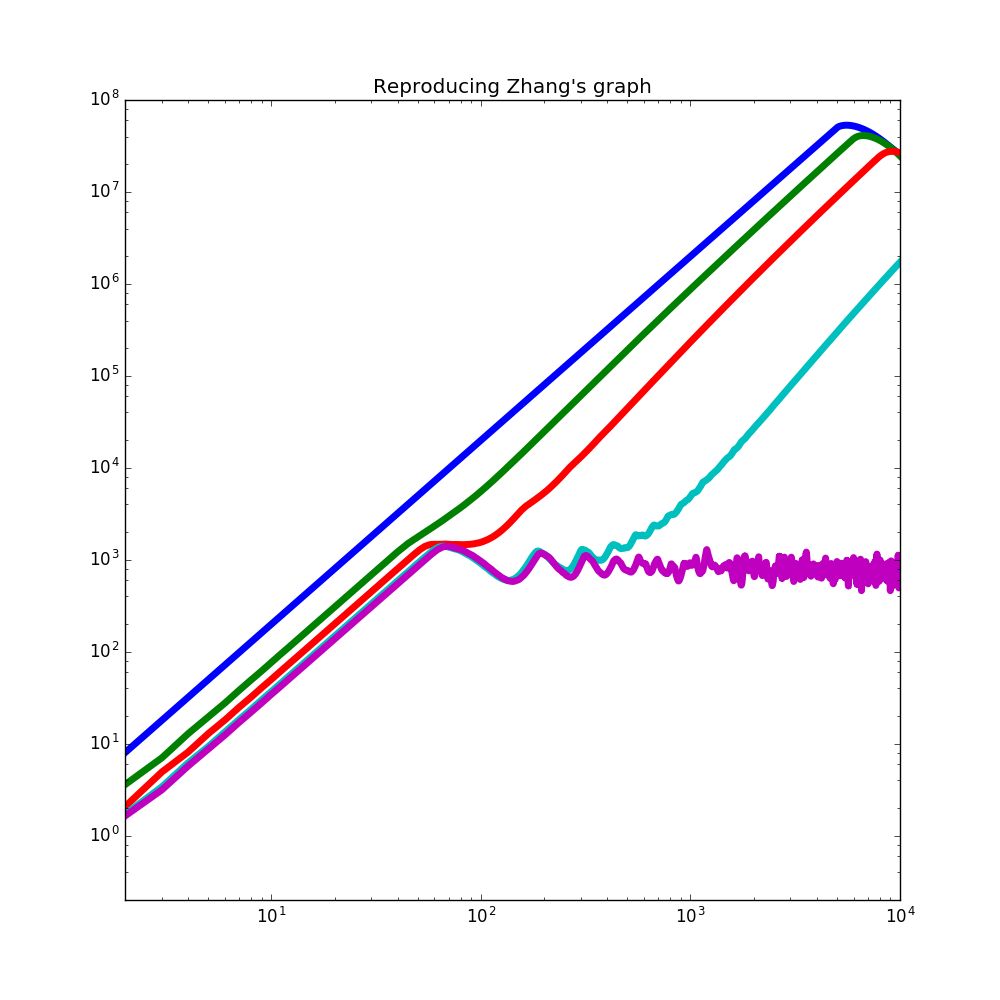
\includegraphics[width=8cm]{zhang.png}
            \caption{波束の分散の時間推移}
        \end{figure}
        \par 特徴として分散が$t^\alpha(\alpha>2)$に比例して増加する現象が見られた。これはZhangが指摘したHeyperdiffusionの特徴と一致している。長時間での分散の値が増加していないのは境界に達した波動関数が反射した影響だと考えられる。
        \par 同じ縮尺のグラフをコンピュータ上で重ねたところ、境界条件の影響を除けば、Zhangの作成したグラフの線の上にQSBのグラフの線が重なることを定性的に確認できた。
        \par また、最小二乗法フフィッティングにより、Zhangの報告している$\alpha$と一致する値が定量的に得られた。各パターンでの$\alpha$を以下に示す。
        \begin{table}[h]
            \begin{tabular}{lcc}
                V&QSB & Zang\\ \hline
                2.0&2.00&2\\
                1.0&2.23&2.2\\
                1.5&2.39&2.4\\
                1.9&2.58&2.6
            \end{tabular}
        \end{table}
    \end{subsection}
\end{section}
\begin{section}{条件設定}
    \par 数値計算におけるパラメータを以下のように設定してQSBによる計算を行った。
    \par 空間の離散化のパラメータは$x\in [-60, 60]$で、$\varDelta x=0.05$のメッシュに自由端境界条件を採用した。時間の離散化パラメータは$t\in [0, 30]$で$varDelata t=0.05$とした。
    \par 初期条件はGauss型波束$\mathrm{std}(x_0, \sigma, x)\mathrm{exp}[ikx]$を使用した。パラメータは平均値$x_0=-15.00$標準偏差$\sigma=6.00$平均波数$k=2.00$に設定した。
    \par 周期ポテンシャルは以下のように設定した。
    \begin{align}
     V(x)=\begin{cases}0&(x<0)\\V_{KP}(x)&(x>0)\end{cases}\nonumber\\
    \end{align}
    \par $V_KP(x)$には3つのパラメータ$a, b, V_0$があるため、本研究で使用するポテンシャルもこれらの3つのパラメータによって完全に決定される。本研究の計算パターンはポテンシャルにのみ依存するため、これらの3つのパラメータのパターンによって各計算パターンは特徴づけられる。
    \begin{subsection}{物理的状況の考察}
        \par 上記の設定は$x<0$の真空領域から、$x>0$の周期ポテンシャル領域に平均波数2.00で入射する波束を想定している。
        \par この平均波数は真空において2.00単位エネルギーを持つ状態で、丸め誤差の範囲内でde Broglie波長$\pi$に対応している。
        \par $V_0=0$の状況では$t=30$の時点で波束中心は$x=45.00$にあり、約片側$2\sigma$が計算範囲内に入る。
        \par $v_0>0$の状況では真空の状況よりも波束の伝搬が遅くなるため、一般に約2.5%の粒子以上の粒子は$x=60$の境界で反射しない。
        \par また、境界で反射した粒子がもう一度$x<0$の領域に侵入する確率は$10^{-10}$を下回ると推定される。
    \end{subsection}
\end{section}
\begin{section}{結果}
    \begin{subsection}{x-tパターン}
        \par 波束の時間発展を$x-t$パターンによって図示した。$x-t$パターンは各時刻における各位置の存在確率を色で表したもので、古典力学で用いられる$x-t$グラフの拡張として捉えることができる。軌跡の傾きは古典的な速度に対応するが、量子力学では量子が確率的な広がりを持つため、軌跡を大まかにしか見取ることはできない。
        \par 縦軸は時刻、横軸は位置を表している。紫の領域の確率密度が最も高く、青緑黄赤の順に低くなっていく。半透明の水色で塗られた領域は壁を意味するが、色jは全て同じで、ポテンシャルの高さとは対応していない。
        \par 以下に挙げられる特徴的なパターンを図示する。
        \begin{itemize}
            \item 全反射
            \item 高次反射波
            \item 高次進行波
            \item 分裂状態
            \item 屈折状態
            \item トラップ状態
            \item 停滞状態
        \end{itemize}
    \end{subsection}
    \begin{subsection}{全反射}
        \begin{figure}[h]
            \centering
            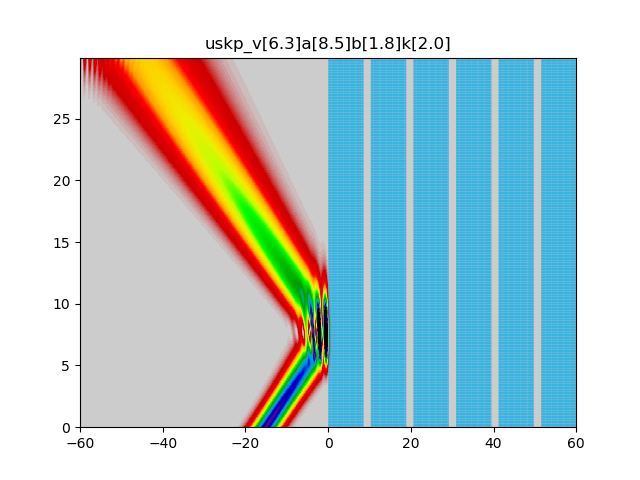
\includegraphics[width=8cm]{zenhansha.png}
            \caption{全反射の例$V_0$=6.3, a=8.5, b=1.8の場合}
        \end{figure}
    \par 壁が厚すぎたり、ポテンシャルが高すぎたりする場合にみられる。ほとんどの波が反射する。
    \end{subsection}
\newpage
    \begin{subsection}{高次反射波}
        \begin{figure}[h]
            \centering
            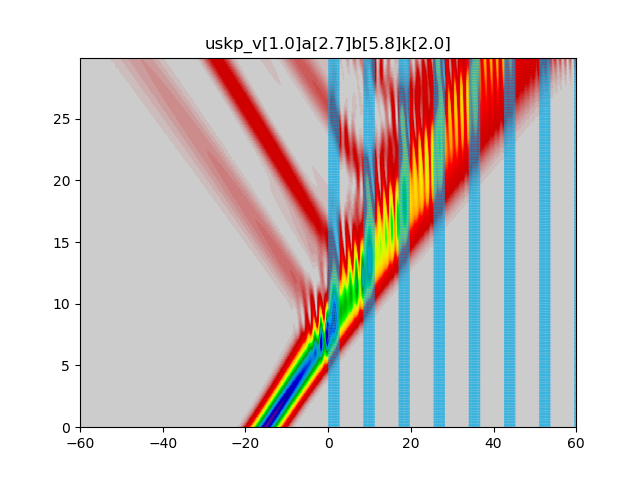
\includegraphics[width=8cm]{tajuhan.png}
            \caption{高次反射波の例$V_0$=1.0, a=2.7, b=5.8の場合}
        \end{figure}
    \par ポテンシャルが$2.0$よりも低く、壁が井戸に比べて非常に薄い場合によくみられる。表層だけでなく2層目や3層目でも反射波束が現れる。ほとんどが2回以上反射しない。
    \par 1つ目の反射波よりもそれ以降の反射波のほうが卓越している場合もみられる。例はポテンシャル1層目内部で反射した2つ目の反射波が最も卓越している。
    \end{subsection}
    \begin{subsection}{高次進行波}
        \begin{figure}[h]
            \centering
            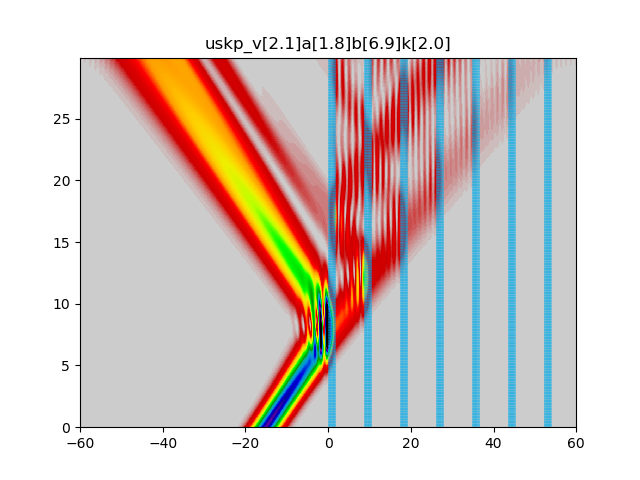
\includegraphics[width=8cm]{tajushin.png}
            \caption{高次進行波の例$V_0$=2.1, a=1.8, b=6.9の場合}
        \end{figure}
    \par 一概にどのような条件でみられるかは見いだされないが、傾向として高次反射波よりもポテンシャルが高い場合に起こりやすい。壁の左側で反射した波束が壁の右側でもう一度反射して、はじめと同じ進行方向へ伝搬する。
    \par すべての壁を透過する波束は時間とともに減衰し、2次進行波やそれ以降の波束が卓越していく。例では20単位時間以降は2次進行波が卓越している。
    \end{subsection}
    \begin{subsection}{分裂状態}
        \begin{figure}[h]
            \centering
            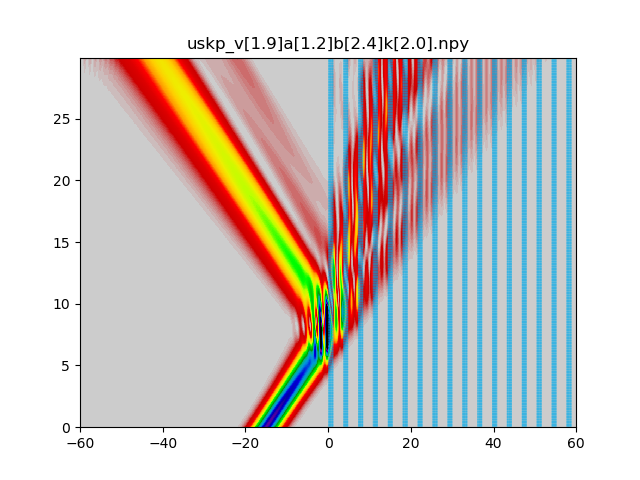
\includegraphics[width=8cm]{bunretsu.png}
            \caption{分裂状態の例$V_0$=1.9, a=1.2, b=2.4の場合}
        \end{figure}
    \par 井戸に対して壁の厚さが同程度の大きさで、周期が5を超えない程度の場合によくみられる。ポテンシャルが高すぎるとみられなくなる。入射波と反射波が重なり合っているため、1次、2次といった進行波の区別は付けられないが、時刻で区切った際に波束が2つ以上の山に分かれる。
    \end{subsection}
    \begin{subsection}{屈折状態}
       \begin{figure}[h]
           \centering
           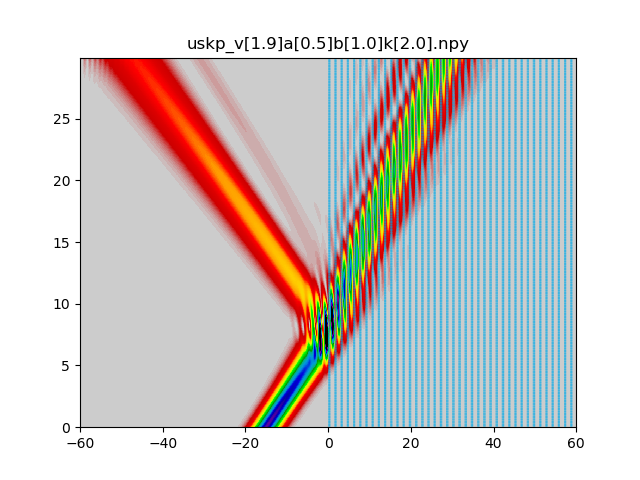
\includegraphics[width=8cm]{kussetsu.png}
           \caption{屈折状態の例$V_0$=1.9, a=0.5, b=1.0の場合}
       \end{figure}
   \par 周期が$1.5$, $3.2$などの場合にみられる。ポテンシャルの高さには関係せず、v=1.9からv=10.0の場合にまでみられた。波束がほぼ完全に一体となってポテンシャル中に入射している。
    \end{subsection}
    \begin{subsection}{トラップ状態}
        \begin{figure}[h]
            \centering
            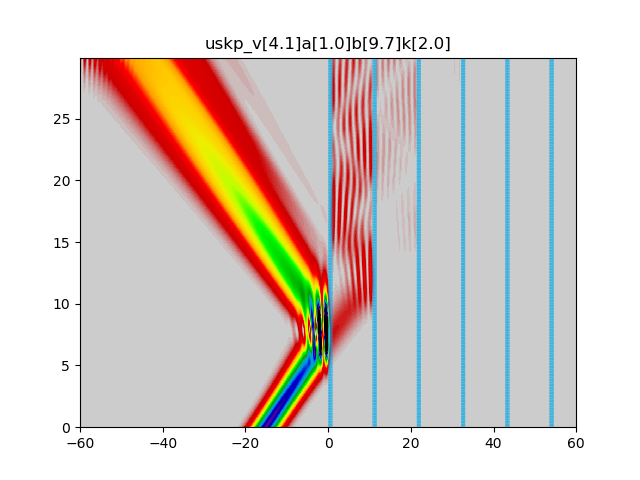
\includegraphics[width=8cm]{trap.png}
            \caption{トラップ状態の例$V_0$=4.1, a=1.0, b=9.7の場合}
        \end{figure}
    \par ポテンシャルが2よりも高く、井戸と比較して壁が薄い場合にみられる。1層と2層の間に波束が入り、出られなくなる。
    \end{subsection}
    \begin{subsection}{停滞状態}
        \begin{figure}[h]
            \centering
            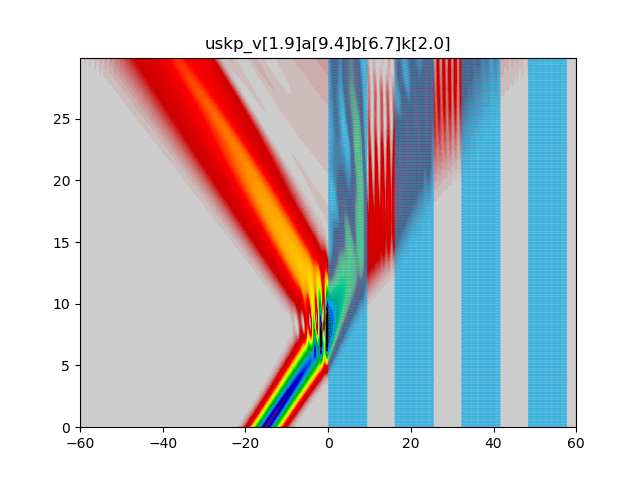
\includegraphics[width=8cm]{tetai.png}
            \caption{停滞状態の例$V_0$=1.9, a=9.4, b=6.7の場合}
        \end{figure}
    \par ポテンシャルが2より低く、壁が5よりも厚い場合によくみられる。例の一層目が顕著だが、ポテンシャル内にとどまり続ける波が存在する。ポテンシャルにとどまる波はポテンシャル表面で反射する場合よりも時間をかけて反射していく。これは、ポテンシャル内の伝搬速度がほぼ0になることで起こる現象だと考えられる。
    \end{subsection}
    \begin{subsection}{反射率と壁の厚さの関係}
        \par t=30の時点で真空領域に滞在している確率を波束の反射率として様々なパターンの反射率を計算した。結果を以下に示す。
        \begin{figure}[h]
            \centering
            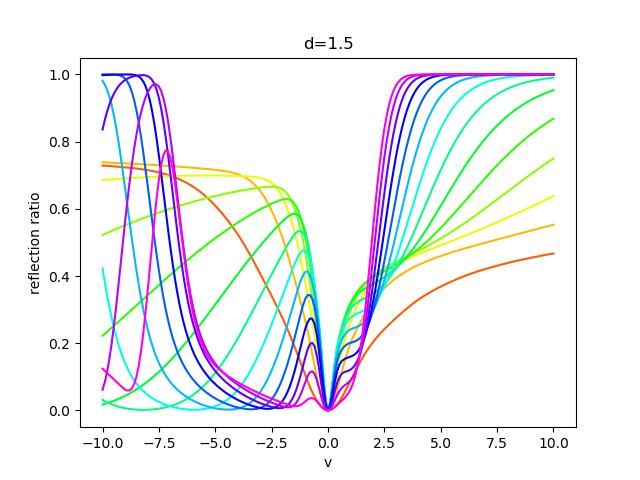
\includegraphics[width=8cm]{hansha.png}
            \caption{周期1.5のポテンシャルの反射率}
        \end{figure}
    \par 曲線の色は1周期における壁の割合を示している。赤から紫にわたって虹のスペクトルと同じ順番で壁の割合が高くなっている。
    \par 注目すべきはV=1.9周辺で、反射率が最も高いものが緑色(壁の割合が50\%程度)であり、赤色(壁の割合が3\%)や紫(壁の割合が97\%)はそれよりも低い。
    \par 古典的な発想ではポテンシャルが高いほど反射率も高くなりそうだが、そのようにはならない。
\newpage
    \par 紫の反射率が低くなる理由は、ポテンシャルの高さが2.0程度と伝搬速度がほぼ0になる場合と近いことだと考えられる。停滞状態のパターンのようにポテンシャル内から出てこなくなっている粒子が一定数存在すると、有限時間での反射率は低く見積もられる。
    \par ポテンシャル領域の滞在時間が高くなることの間接的証拠として、箱型ポテンシャルの場合を示す。箱型ポテンシャルの定常状態における真空領域とポテンシャル領域の確率密度の比は以下のようになる。
     \begin{figure}[h]
        \centering
        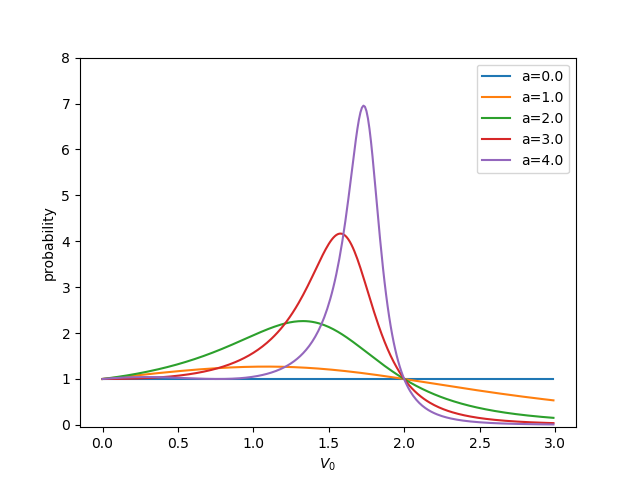
\includegraphics[width=8cm]{hako_in.png}
        \caption{真空領域の滞在確率/ポテンシャル領域の滞在確率}
    \end{figure}
    \par 横軸はポテンシャルの高さ、縦軸は真空領域の確率密度/ポテンシャル領域の確率密度を表している。縦軸が1を超えた場合、粒子が見いだされる確率密度はポテンシャル領域のほうが高いことを意味している。
    \par 系のエネルギーはシミュレーションと同様に2に設定している。
    \par $V_0<2$の領域ではポテンシャル内のほうが確率密度が高くなっていることがわかる。また、$V_0$が2よりも少しだけ小さいときに現れるピークは$a$が大きくなるほど鋭くなることがわかる。
    \par よって、入射エネルギーよりも少しだけ低いポテンシャルでは、aの値が大きくなるごとに滞在時間が増えていくことがいえる。停滞状態のパターンから、Kronig-Pennyポテンシャルでも同様の傾向があると考えられる。
    \end{subsection}
\end{section}
\newpage
\appendix
\begin{section}{Blochの定理の簡単な証明}
    \par ハミルトニアンHに以下の条件を課す。$T_d$は移動距離$d$の並進演算子。
    \begin{align}
     [T_d,H]=0\nonumber\\
    \end{align}
    \par これは並進対称性を表している。これにより、固有状態$\phi$は$d$の整数倍の周期を持ち、$H$と$T_d$の同時固有状態になる。並進演算子の固有状態は1の整数乗根になる。
    \begin{align}
     T_d\phi=A\phi\nonumber\\
        (T_d)^n\phi=A^n\phi=\phi\nonumber\\
        A=\mathrm{e}^{i2\pi/n}=\mathrm{e}^{iKd}\nonumber\\
        K=\frac{2\pi}{n d}
    \end{align}
    \par $\phi$の周期を$nd$とした。ここで以下の関数$u$を考える。
    \begin{align}
     u(x) &= \mathrm{e}^{iKx}\phi(x)\label{ux}\nonumber\\
    \end{align}
    \begin{align}
     T_d u(x) &= \mathrm{e}^{iK(x-d)}\mathrm{e}^{iKd}\phi(x)\nonumber\\
        T_d u(x) &= \mathrm{e}^{iKx}\phi(x)=u(x)
    \end{align}
    \par よって$u(x)$は周期$d$を持つ周期関数だということが分かる。
    \par $u(x)$の定義を変形すればBlochの定理を証明したことになる。
    \begin{align}
     \phi(x) = \mathrm{e}^{-iKx}u(x)\nonumber\\
    \end{align}
    \par $K$を三次元に拡張したものは逆格子ベクトルと呼ばれる。
\end{section}
\begin{section}{Kronig-Pennyモデルのエネルギーバンド構造の簡単な計算方法}
    \par 井戸と壁のSchrödinger方程式は単純な単振動になるため、エネルギーを$\varepsilon$としたとき以下のような解になる。
    \begin{align}
     \phi_{well}(x)=W^+\mathrm{e}^{+ikx}+W^-\mathrm{e}^{-ikx}\nonumber\\
        \phi_{barrier}(x)=B^+\mathrm{e}^{+iqx}+B^-\mathrm{e}^{-iqx}\nonumber\\
        k=\sqrt{2m\varepsilon}\nonumber\\
        q=\sqrt{2m(\varepsilon - V_0)}
    \end{align}
    \par $W^+$,$W^-$,$B^+$,$B^-$は振幅を表す定数。
    \par $\phi(x)$に一回微分までの連続性を課すと、井戸と壁の境界で以下の条件が必要となる。
    \begin{align}
     \begin{pmatrix} 1 & 1 \\ 1 & -1 \end{pmatrix}\begin{pmatrix} W^{ + } \\ W^{ - } \end{pmatrix}=\begin{pmatrix} 1 & 1 \\ \rho & -\rho \end{pmatrix}\begin{pmatrix} B^{ + } \\ B^{ - } \end{pmatrix}\nonumber\\
    \end{align}
    \begin{align}
     \begin{pmatrix} \mathrm{e}^{ika} & \mathrm{e}^{-ika} \\ \mathrm{e}^{ika} & -\mathrm{e}^{-ika} \end{pmatrix}\begin{pmatrix} W^{+} \\ W^{-} \end{pmatrix}=\begin{pmatrix} \mathrm{e}^{iqa} & \mathrm{e}^{-iqa} \\ \rho\mathrm{e}^{iqa} & -\rho \mathrm{e}^{-iqa} \end{pmatrix}\begin{pmatrix} B^{+} \\ B^{-} \end{pmatrix}\nonumber\\
    \end{align}
    \par ここで$\rho=q/k$。
    \par Blochの定理を上式の左辺に使うと以下の置き換えをすることが出来る。
    \begin{align}
        \mathrm{e}^{ika}\rightarrow\mathrm{e}^{ikb}\mathrm{e}^{-iKd}\\
        \mathrm{e}^{-ika}\rightarrow\mathrm{e}^{-ikb}\mathrm{e}^{-iKd}
    \end{align}
    \end{section}
    簡略のために以下の置換えをする。
    \begin{align}
     H&=\begin{pmatrix} 1 & 1 \\ 1 & -1 \end{pmatrix}\nonumber\\
        \alpha &=\begin{pmatrix} 1 & 0 \\ 0 & \rho  \end{pmatrix}\nonumber\\
        K_x&=\begin{pmatrix} \mathrm{e}^{ikx} & 0 \\ 0 &  \mathrm{e}^{-ikx} \end{pmatrix}\nonumber\\
        Q_x&=\begin{pmatrix} \mathrm{e}^{iqx} & 0 \\ 0 &  \mathrm{e}^{-iqx} \end{pmatrix}\nonumber\\
        \mathbf{W}& = \begin{pmatrix} W^{+} \\ W^{-} \end{pmatrix}\nonumber\\
        \mathbf{B}& = \begin{pmatrix} B^{+} \\ B^{-} \end{pmatrix}
    \end{align}
    ちなみに、HはHadamard行列として知られている。
    置き換えをすると以下のような式が得られる。
    \begin{align}
     H \mathbf{W} - H \alpha \mathbf{B} = 0\nonumber\\
        \mathrm{e}^{-iKd} K_b H \mathbf{W} - Q_a H \alpha \mathbf{B} = 0
    \end{align}
    整理すると以下のような方程式が得られる。
    \begin{align}
     \begin{pmatrix} E & \alpha  \\ E & { e }^{ iKd }H^{ -1 }K_{ b }^{ -1 } Q_{ a }H\alpha  \end{pmatrix}\begin{pmatrix} \mathbf{ W } \\ \mathbf{ B } \end{pmatrix}=0\nonumber\\
    \end{align}
    ここで$E$は2次の単位行列。
    トリビアルでない解は行列部分が0となるときに現れる。4行4列の行列式を求める手続きは煩雑だが、余因子展開を繰り返せば必ず展開できる。幸い、今回は単位行列が現れることを利用すれば、実質的に現れる項は4項だけとなる。

\begin{section}{定常状態の計算}
    \par 数値計算で用いたポテンシャルにおける定常解は転送行列によって扱うことが出来る。
    \begin{align}
     V(x)=\begin{cases}0&(x<0)\\V_{KP}(x)&(x>0)\end{cases}\nonumber\\
    \end{align}
    \par Schrödinger方程式の解はKronig-Pennyモデルの計算と同じ形になる。連続の条件を課すと、以下の境界条件が成立する。
    \begin{align}
     K_{dn} H \mathbf{W_n} = Q_{dn} H \alpha \mathbf{B_n}\nonumber\\
        K_{a} K_{dn} H \mathbf{W}_{n+1} = Q_a Q_{dn} H \alpha \mathbf{B}_n
    \end{align}
    \par 前章で用いた置き換えを使った。$W_n$, $b_n$は0から数えて原点からn周期目の井戸、壁における振幅を表している。
    \par 上式から井戸の振幅についての漸化式を作ると以下のようになる。
    \begin{align}
     \mathbf{W}_{n+1}= H^{-1} K_{dn}^{-1} K_a^{-1} Q_a K_{dn} H \mathbf{W}_n\nonumber\\
    \end{align}
    \par ちなみに、一般項は以下のようになる。
    \begin{align}
     \mathbf{W}_n = H^{-1} \left( K_b Q_a \right)^n H \mathbf{W}_0\nonumber\\
    \end{align}
    \par 初項$W_0$を漸化式の係数部分$A = H^{-1} K_{dn}^{-1} K_a^{-1} Q_a K_{dn} H$の固有ベクトル$A_1$, $A_2$で展開する。ここで、固有値$a_1$, $a_2$ には$|a_1|<|a_2|$の関係があることにする。
    \begin{align}
     \mathbf{W}_n = c_1 A_1 + c_2 A_2\nonumber\\
      W_0 = A^{-n} W_n = c_1 a_1^{-n} A_1 + c_2 a_2^{-n} A_2
    \end{align}
    \par ここで、$n \rightarrow \infty$の場合を考えると、$|a_1|^{-n}>>a_2^{-n}$となり、$W_0$の主成分は$A_1$となる。
    \par $A_1$における進行波と後退波の比をとれば、反射率を得ることが出来る。
\end{section}
\begin{section}{QSBのクラス構成}
    QuantumSketchBookのデータ構造はクラスとしてまとめられている。以下に主要なクラスを示す。
    \begin{itemize}
        \item Mesh:離散化のデータを保持する
        \item Context:Meshを配布する
        \item Field:空間に依存する物理量を表す
        \item Potential:ポテンシャルを表す
        \item State:初期状態を表す
        \item Hamiltonian:ハミルトニアンを表す
        \item Schrodinger:初期値問題を計算する
    \end{itemize}
    \par また、QSB独自概念としてplottableという概念がある。これはQSB付属のplot()関数によって適切なグラフが出力される性質を持つことを指す。
    \begin{subsection}{Mesh}
        \par 時空間の離散化に関するデータを保持する。様々なオブジェクトが離散化の際にこのクラスを利用するため、自動でMeshにアクセスできるよう、Contextクラスが提供されている。
        \par 異なったMeshによる計算が行われそうになった場合、MeshErrorが送出される。
        \par 不慣れな利用者による直接のインスタンス化(具体的なデータを入力してテータ構造を生成すること)は推奨されない。
    \end{subsection}
    \begin{subsection}{Context}
        \par Meshの配布を行う。QSBのほとんどのクラスはContextが自動生成したMeshを自動で受け取ることが出来るように作成されているため、利用者はこのContextをインスタンス化するだけで、離散化に関する処理は考えなくても良くなる。
        \par 複数のContextが存在する場合、最後にインスタンス化されたContextの情報が優先される。Contextの有効範囲を明示化出来るようwith構文によるコンテキストマネージャとしての使用法がサポートされている。
        \par Context.\_\_enter\_\_()メソッド(コンテキストマネージャとして使用された際にpython内部で呼ばれるメソッド)はMeshを返す。
    \end{subsection}
    \begin{subsection}{Field}
        \par 空間に依存する物理量を表す。引数には配列と関数のどちらも受け取ることができる。ただし、配列の要素数と空間メッシュの数が一致しない場合ValueErrorを送出する。
        \par Field内部で各位置での値の情報をMeshと結びつけて保持する。Meshが引数として与えられない場合、Contextから自動的に情報を受け取る。Contextが存在しない場合はMeshContextErrorが送出される。
        \par 抽象クラスとして設計さているため、このクラスを直接インスタンス化することは推奨されない。
    \end{subsection}
    \begin{subsection}{Potential}
        \par ポテンシャルの情報を保持する。Fieldのサブクラスのため、配列と関数を受け取ることが出来る。
        \par スカラー倍とポテンシャル同士の加減がサポートされている。
        \par plottableであるため、Plot(some\_potential)とすれば、グラフを作成できる。
        \par 具体的なPotentialを構成するための関数(box(), step(), kp()など)がいくつか用意されている。
    \end{subsection}
    \begin{subsection}{State}
        \par 初期状態に関する情報を保持する。Fieldのサブクラスのため、配列と関数を受け取ることが出来る。
        \par 確率分布に従う乱数生成を行うことが出来る。
        \par plottableであるため、Plot(some\_state)とすれば、グラフを作成できる。
        \par Gauss型波束のStateを構成するための関数gaussian\_state()が用意されている。
    \end{subsection}
    \begin{subsection}{Hamiltonian}
        \par Potentialを受け取って、ハミルトニアン演算子を保持する。
        \par 行列要素は疎行列によって保持されているため、メモリ効率、時間効率ともに効率化されている。
        \par 境界条件の指定はこのクラスによって行われる。物理的には時空を管理するMeshに保持させるべき情報だが、同様のMeshを異なった境界条件で計算する可能性が高いことから、全てのデータの基礎となっているMeshではなく、比較的変更しやすいHamiltonianに保持させる形になっている。
    \end{subsection}
    \begin{subsection}{Schrodinger}
        \par 初期値問題の求解を行う。HamiltonianとStateを受け取ってSchrödinger方程式の数値解を保持する。
        \par 数値解は初めてSchrodinger.solution()メソッドが呼び出されたときに計算され、キャッシュされる。よって、二回目以降の呼び出しは高速になる。 また、Schrodeingerはiterbleであり、各ステップでの解を順々に返すことが出来る。この機能はMeshが巨大すぎてメモリ消費が激しいときに有効な方法として設計されている。
        \par plottableであり、plotするとx-tパターンを生成する。
    \end{subsection}
\end{section}
\begin{section}{サンプルコード}
    import QuantumSketchBook as QSB\\\\
        with QSB.Context(0, 1, 0.01, 0, 1, 0.01) as mesh:\\
        \ \ \ \  my\_potential = QSB.potential(lambda x: x ** 2)\\
        \ \ \ \  my\_state = QSB.gaussian\_state(0, 2, 0)\\
        \ \ \ \  my\_hamiltonian = QSB.Hamiltonian(my\_potential)\\
        \ \ \ \  my\_schrodinger = QSB.Schrodinger(my\_hamiltonian,\  my\_state)\\
        \ \ \ \  QSB.plot(my\_schrodinger)
\end{section}
\end{document}
